\documentclass[12pt, utf8, hyperref]{ctexart}
% \usepackage{ctex}
\usepackage{graphicx}
\usepackage{float}

\hypersetup{
    colorlinks=true,
    linkcolor=black
} %set link in table of contents to black (default red)

\begin{document}
\begin{titlepage}
\centering
\vspace*{\stretch{1}}

\Huge{\textbf{THCO MIPS32e \\ 系统设计与实现报告}}

\vspace{\stretch{2}}

\begin{table}[h]
\centering
\Large
\begin{tabular}{lll}
计65 & 李依林 & 2016011502 \\
计65 & 张岱墀 & 2016011364 \\
计65 & 王琛 & 2016011360
\end{tabular}
\end{table}

\vspace{\stretch{1}}
\normalsize December, 2018
\end{titlepage}


\cleardoublepage

\tableofcontents

\newpage
\section{实验目标}
本实验是计算机组成原理课程大实验。在本次试验中,我们设计并且实现了一个基本符合冯•诺伊曼架构的“计算机”。在THINPAD教学计算机硬件平台上,完成了一个基于MIPS32指令标准的CPU,并且能够运行监控程序。

本组实现的功能如下:
\begin{itemize}
    \item 基于THINPAD教学计算机的MIP32指令流水CPU
    \item 使用基本存储、扩展存储、Flash完成实验,并且支持VGA显示
    \item 使用数据旁路的机制,解决了结构冲突、数据冲突和控制冲突
\end{itemize}

\section{主要模块设计}
我们的CPU实现遵守了MIPS的5级流水线架构,一个周期分为if, id, ex, mem, wb五个阶段,并在每两个阶段之间加入 流水线寄存器,用来保存一个流水段传送到下一个流水段的所有数据和控制信息。
\subsection{pc}
PC模块是取指阶段,目的是给出下一条指令的地址。当流水线暂停时,可以从控制模块给出PC。在流水线正常执行时,每个周期PC的值会加4,表示下一条指令的地址。同时,PC模块还支持分支跳转指令的指令。

\subsection{if}
根据pc传来的指令地址从Rom中读取相应的指令,具体实现时将其放入了ctrl模块中。

\subsection{if\_id}
if\_id是暂存模块。本模块暂存取指阶段取得的指令,以及指令的pc值,并且在下一个时钟上升沿传递到译码阶段。

\subsection{id}
id模块的作用是对指令进行译码,获取操作数,产生控制信号并且传给后面的模块。具体如下:
\begin{enumerate}
    \item 根据指令的编号,判断指令输入哪一大类的指令(包括逻辑类型、算术类型、移位类型等等)。每个大类型再分为一些小类型,因此判断完大类之后再判断其属于哪一个具体的类型。再根据指令的类型决定要读写哪些个寄存器。读取寄存器的值之后,将读取的值、是否写入要写入寄存器、要写入的寄存器的编号传入ex阶段。
    \item 本阶段还要解决数据前推的问题。一是来自执行阶段的运算结果,包括是否应该写入寄存器、写入寄存器的编号、写入的数据。二是来自访存阶段指令的运算结果,包括处于访存阶段的指令是否要写目的寄存器、写入目的寄存器的值、写入目的寄存器的地址。
\end{enumerate}

\subsection{regfile}
regfile模块用verilog实现了MIPS32的32个32位寄存器,可以同时进行两个寄存器的读操作以及一个寄存器的写操作。

\subsection{id\_ex}
id\_ex模块介于id和ex之间,作用是将译码阶段取得的运算类型、运算子类型、运算数以及寄存器相关信息暂存,等到下一个时钟上升沿传递给ex阶段进行运算。

\subsection{ex}
ex模块获得id\_ex传递的运算类型、操作数等信息,进行执行操作。如果是算数和逻辑指令则进行相应的运算即可,如果是分支或跳转则无需操作,如果是load/store指令,计算访存的地址,对于移动指令,完成对HILO寄存器访问的修改和数据冲突的解决。

另外,此阶段还需要将计算的结果前推到id阶段来处理数据冲突,并且接收mem模块以及mem\_wb模块前推来的数据。

\subsection{ex\_mem}
ex\_mem是暂存模块,作用时存储执行阶段获得的运算结果及要写入的寄存器相关信息,并在下个时钟上升沿传递到流水线下一阶段。

\subsection{mem}
mem阶段是访存阶段,作用是访问内存,根据前面的地址得到相应的数据。另外,此阶段还要将数据前推给id和ex阶段以处理读后写问题。

\subsection{mem\_wb}
mem\_wb模块的作用是得到访存阶段的运算结果,在下一个时钟周期内写入寄存器。

\subsection{ctrl}
ctrl模块用于控制流水线运行,响应流水线暂停请求,可以控制各个阶段的运行状态,保证时钟周期的正确性。

\subsection{hilo\_reg}
hilo\_reg包含了hi、lo寄存器,用于进行乘法和除法相应的运算,保存结果。其中,hi寄存器保存结果的高32位,lo保存低32位。同时,还可以对其进行查询和写入。

\subsection{flash}
由于断电后程序不丢失,flash可用于自启,按rst键后会自动从Flash中读出内容放到内存中,从而启动监控程序。读Flash时,先将地址准备好,然后将we 拉低,进入读模式,再将we拉高,oe拉低,读出对应位置数据。这一过程用状态机实现。

在按 rst 键后,暂停CPU的一切功能,然后从0地址开始读Flash。每次读取16个比特。

\subsection{vga}
vga包括行同步信号和场同步信号,挨个扫描屏幕上的像素点,其中像素信息从内存中获得,为8位rgb值,分别为红色3位,绿色3位,蓝色2位。基于vga,我们实现了如下功能:
\begin{itemize}
    \item 显示一张完整的图片
    \item 通过板子上的按钮控制方向,实现了一个简易的推箱子游戏
    \item 屏幕上的计数器,按clk键时进行计数
\end{itemize}
\begin{figure}[H]
    \centering
    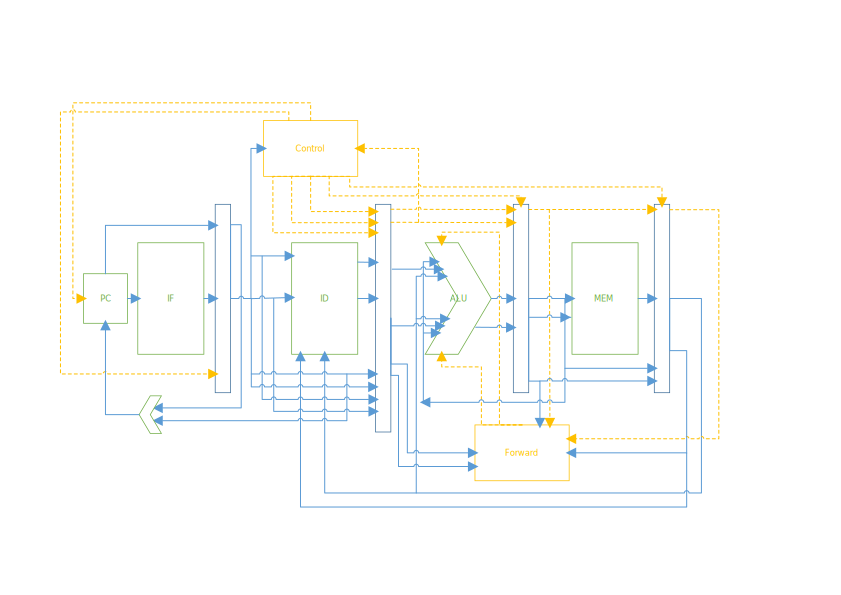
\includegraphics[width=1.5\textwidth, angle=270]{screenshots/datapath.png}
    \caption{数据通路图}
\end{figure}
\newpage

\section{实验结果}
\subsection{监控程序测试}

\begin{figure}[H]
    \centering
    \includegraphics[width=0.55\textwidth]{screenshots/r.png}
    \caption{r型指令显示寄存器信息}
\end{figure}

\begin{figure}[H]
    \centering
    \includegraphics[width=0.55\textwidth]{screenshots/u.png}
    \caption{u指令向内存中写入程序}
\end{figure}

\begin{figure}[H]
    \centering
    \includegraphics[width=0.7\textwidth]{screenshots/d.png}
    \caption{d指令显示内存数据}
\end{figure}

\begin{figure}[H]
    \centering
    \includegraphics[width=0.7\textwidth]{screenshots/性能测试.png}
    \caption{22.5M时钟测试}
\end{figure}

\begin{figure}[H]
    \centering
    \includegraphics[width=0.7\textwidth]{screenshots/div.png}
    \caption{除法指令测试}
\end{figure}

\begin{figure}[H]
    \centering
    \includegraphics[width=0.7\textwidth]{screenshots/mul.png}
    \caption{乘法指令测试}
\end{figure}

\subsection{外设展示}
\begin{figure}[H]
    \centering
    \includegraphics[width=0.7\textwidth]{screenshots/sokoban.JPG}
    \caption{推箱子小游戏}
\end{figure}

\begin{figure}[H]
    \centering
    \includegraphics[width=0.7\textwidth]{screenshots/counter.JPG}
    \caption{计数器}
\end{figure}

\begin{figure}[H]
    \centering
    \includegraphics[width=0.7\textwidth]{screenshots/image.JPG}
    \caption{显示图片}
\end{figure}

\section{感想}
\subsection*{李依林同学}
回顾三周余的造机经历,心情复杂。感到欣慰的是和同伴们并肩作战,共同完成了预期的大部分目标,完成了一个有一定复杂度的硬件系统;感到遗憾的是并非没有努力,但本可以做得更好。

和同伴们共同完成了基本数据通路的实现后,我主要负责实现访存、解决结构冲突、以及整合同伴完成的外设模块的工作。就基本功能而言,我们主要受到两个问题的困扰:一是端序(我们首先实现的是MIPS经典的大端序,且给出的汇编代码也有错误),二是时钟(例如,我们使用手动分频的12.5M时钟运行时有错误,但改用PLL便能提高到近25M)。第一个问题解决后,能以11.0592M顺利运行kernel程序,离交付还有最多近一周的时间,一度感到时间还算充足;此时认为可以先保证功能的正确性,最后再提高主频(从软件角度看这恐怕是很合理的,然而……)。但最后几天对代码最谨慎的优化几乎都会造成运行结果从正确变为错误,未曾想最主要的问题不在于流水线,而恰恰在于时钟!这也间接导致我们最后没有充分的时间调试已经通过仿真的异常部分,留下了遗憾。

个人认为,我们对于基础功能的实现无可厚非:经过重构,解决结构冲突部分应该是优雅且高效的,访存和模块间整合未必非常高效但也合乎规范。而主要失误有二:一是前期对project-specific信息的调研不够充足,例如前面提到的时钟,又例如即便不通过异常机制也有一些控制外设的巧workaround;二是没有尽早地解决时钟问题。算是为增长人生经验付出的学费吧。

\subsection*{张岱墀同学}
本次三周造机过程中,前期完成了基本数据通路的绘制,和队友共同完成了流水线各个模块的代码以及相关指令的实现,完成了flash模块的代码实现,串口部分逻辑,以及VGA外设的图片显示和推箱子的相关扩展。

但我们的工作中也有很多不足。时间安排方面,感觉这次造机的工作量全部堆积在最后一周,可能前期对于时间分配还是多多少少出了些问题。工作细节方面,在完成配合各个模块对接上板时,对于助教所要求的虚拟地址映射以及板子上各个部分配合工作这方面理解不够导致当初滞留在这很久。往后还是着手干活前应该更认真思考整体工作。外设扩展方面,在完成外设模块后着手于外设做扩展时,由于思考方向有点错误,导致外设的扩展和流水线的关系没有希望中的那么紧密。这是考虑扩展实现方法的时候的疏忽。

三周造机时间过的很快,在东主楼也度过了一段难忘的时光。和队友一起为了造出一台计算机一起奋斗;在东主的很多同学同一目标而奋斗的氛围;助教和老师的帮助。可能造出来的这个32位板并不算多么完美无缺,但很纯粹地去做一件事这个过程,过程中一步一步完成了每一步时的喜悦以及最后获取的成就感,这些确实是整个造机三周中很难忘的回忆。

\subsection*{王琛同学}
三周的造机历程不知不觉已经过去半个月了。从大一入学就听说了贵系这门“奋战三星期,造台计算机”的神课,不知不觉就轮到了自己。尽管中间有些坎坷,身体也出现了不适,但是最终我们还是顺利完成了要求。在这里我尤其要感谢和我并肩作战的队友,悉心帮忙的老师和助教,以及一起讨论的其他组同学。

回想起造机的过程,有点像过山车一般。在我和同伴完成了基本的指令集、加上了串口和访存之后,使用了11M的时钟,没出什么大的问题就跑出了监控程序,我们一时间感觉进度还算不错。后来我们的精力主要转为了外设,然而到最后提升主频时却频繁出现问题,使用了各种办法都无法提高。在交付的前一天网上使用PLL才勉勉强强跑到了25M,算是比较慢的一个主频吧。这件事也给了我一个深刻的教训。另外,在做外设扩展时,我们的思考方式也出了一些问题,只是想着用硬件描述语言去实现功能,却没有尝试直接写一个软件程序;另外,我们也没有将外设和流水线紧密联系在一起,有些脱离我们造的“计算机”。

总之,不论最后结果如何,能够顺利完成我深感欣慰。如果规划能够更加完整,可能有些问题就不会出现,我们的实现也会更完整一些。在此再次感谢我的队友!

\end{document}
